% ---------------------------------------------------------------------------
% Vista de conjunto de la plataforma: del software del PS a los periféricos,
% con cada bloque marcado con el objetivo específico al que responde.
% Fuente del PDF que incluye la memoria (capítulo 1).
%
% El bloque de transporte muestra las tres variantes y no solo la MCDMA: las
% placas CDHS y AOCS se validaron sobre la variante GPIO, así que dibujar la
% MCDMA alimentando todas las placas no sería cierto.
%
% Sobre la planta: las placas van apiladas en filas y no en tres columnas. Así
% el dibujo es más estrecho, el factor de escala hasta el ancho de caja sube y
% la letra se lee; a cambio ocupa más alto. Los rellenos van más saturados que
% en el resto de diagramas para que el azul y el verde se distingan en papel.
%
% Compilar:  pdflatex diagrama_vision_general.tex
% ---------------------------------------------------------------------------
\documentclass[border=8pt]{standalone}
\usepackage[utf8]{inputenc}
\usepackage[T1]{fontenc}
\usepackage{lmodern}
\usepackage{tikz}
\usetikzlibrary{arrows.meta, calc, decorations.pathreplacing}

\definecolor{cPropio}{HTML}{2A78D6}   % azul: lógica de diseño propio
\definecolor{cIP}{HTML}{EDA100}       % ámbar: IP de terceros
\definecolor{cExt}{HTML}{1BAF7A}      % aguamarina: software y hardware externo
\definecolor{cRef}{HTML}{8A8A85}      % gris: líneas, bandas y contornos

\begin{document}
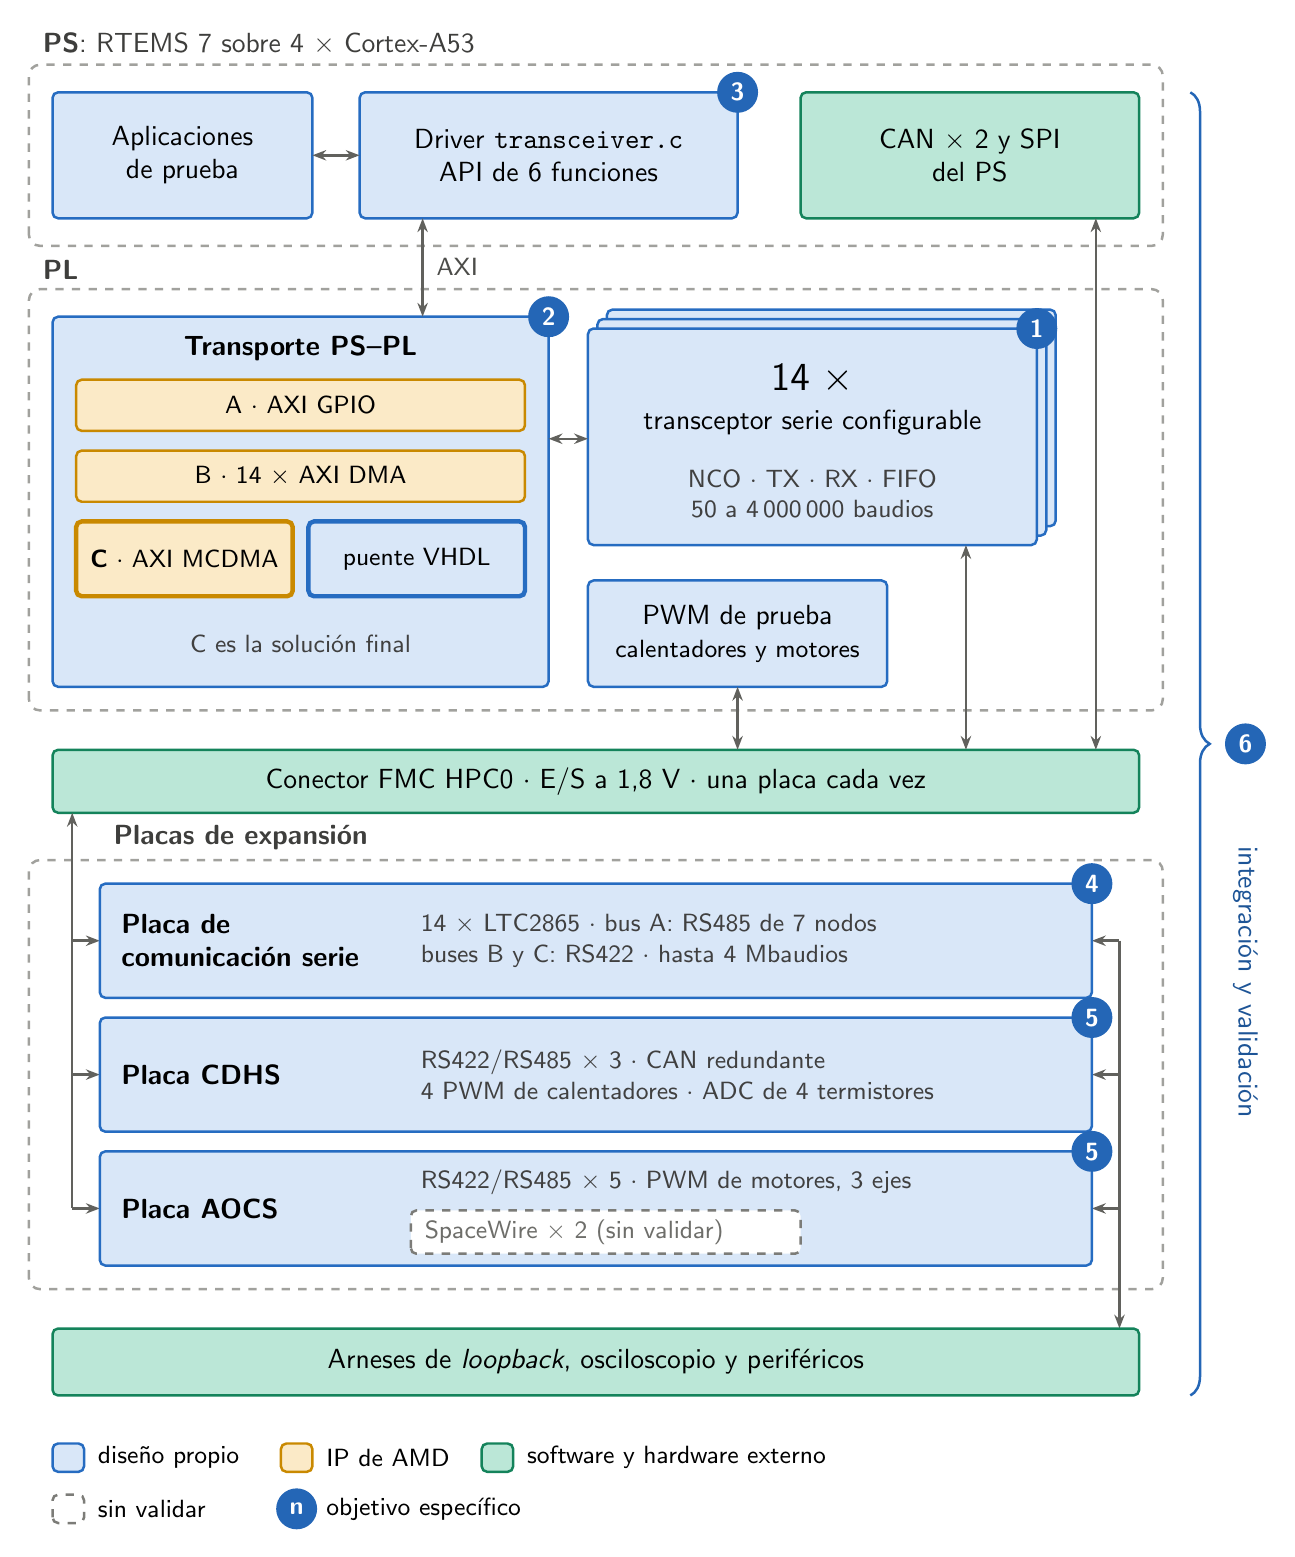
\begin{tikzpicture}[
    x=1cm, y=1cm, font=\sffamily\normalsize,
    blk/.style={draw=cPropio!90!black, line width=0.9pt, rounded corners=2pt,
                fill=cPropio!18},
    ip/.style={draw=cIP!85!black, line width=0.9pt, rounded corners=2pt,
               fill=cIP!22},
    ext/.style={draw=cExt!75!black, line width=0.9pt, rounded corners=2pt,
                fill=cExt!30},
    nov/.style={draw=cRef!90!black, dashed, line width=0.9pt, rounded corners=2pt,
                fill=white},
    band/.style={draw=cRef!80, dashed, line width=0.9pt, rounded corners=4pt},
    arr/.style={-{Stealth[length=5pt]}, line width=0.9pt, cRef!70!black},
    bus/.style={{Stealth[length=5pt]}-{Stealth[length=5pt]},
                line width=0.9pt, cRef!70!black},
    lbl/.style={font=\sffamily\small, inner sep=2pt},
    sub/.style={font=\sffamily\small, text=black!75, inner sep=2pt},
    bandlbl/.style={font=\sffamily\normalsize, text=cRef!45!black, inner sep=2pt},
    badge/.style={circle, fill=cPropio!85!black, text=white,
                  font=\sffamily\small\bfseries, inner sep=0pt,
                  minimum size=5.2mm},
    leg/.style={font=\sffamily\small, inner sep=2pt},
]

% ===================== Bandas =====================
\draw[band] (0.00,15.25) rectangle (14.40,17.55);
\node[bandlbl, anchor=south west] at (0.10,17.60)
      {\textbf{PS}: RTEMS 7 sobre 4 $\times$ Cortex-A53};

\draw[band] (0.00,9.35) rectangle (14.40,14.70);
\node[bandlbl, anchor=south west] at (0.10,14.75) {\textbf{PL}};

\draw[band] (0.00,2.00) rectangle (14.40,7.45);
% El rótulo se aparta a la derecha de la guía que baja del conector.
\node[bandlbl, anchor=south west] at (1.00,7.50) {\textbf{Placas de expansión}};

% ===================== PS =====================
\draw[blk] (0.30,15.60) rectangle (3.60,17.20);
\node[align=center] at (1.95,16.40) {Aplicaciones\\de prueba};

\draw[blk] (4.20,15.60) rectangle (9.00,17.20);
\node[align=center] at (6.60,16.40) {Driver \texttt{transceiver.c}\\API de 6 funciones};
\node[badge] at (9.00,17.20) {3};

\draw[ext] (9.80,15.60) rectangle (14.10,17.20);
\node[align=center] at (11.95,16.40) {CAN $\times$ 2 y SPI\\del PS};

\draw[bus] (3.60,16.40) -- (4.20,16.40);

% ===================== PL: transporte PS--PL =====================
\draw[blk] (0.30,9.65) rectangle (6.60,14.35);
\node[font=\sffamily\normalsize\bfseries] at (3.45,13.95) {Transporte PS--PL};
\node[badge] at (6.60,14.35) {2};

\draw[ip] (0.60,12.90) rectangle (6.30,13.55);
\node[lbl] at (3.45,13.225) {A $\cdot$ AXI GPIO};

\draw[ip] (0.60,12.00) rectangle (6.30,12.65);
\node[lbl] at (3.45,12.325) {B $\cdot$ 14 $\times$ AXI DMA};

% La variante final va con trazo grueso para distinguirla de las otras dos.
\draw[ip, line width=1.6pt] (0.60,10.80) rectangle (3.35,11.75);
\node[lbl] at (1.975,11.275) {\textbf{C} $\cdot$ AXI MCDMA};
\draw[blk, line width=1.6pt] (3.55,10.80) rectangle (6.30,11.75);
\node[lbl] at (4.925,11.275) {puente VHDL};
\node[sub] at (3.45,10.20) {C es la solución final};

% ===================== PL: transceptores =====================
% Dos sombras desplazadas sugieren la pila de catorce instancias.
\draw[blk] (7.34,11.69) rectangle (13.04,14.44);
\draw[blk] (7.22,11.57) rectangle (12.92,14.32);
\draw[blk] (7.10,11.45) rectangle (12.80,14.20);
\node[align=center] at (9.95,13.30)
      {{\Large 14 $\times$}\\[2pt]transceptor serie configurable};
\node[sub, align=center] at (9.95,12.10)
      {NCO $\cdot$ TX $\cdot$ RX $\cdot$ FIFO\\50 a 4\,000\,000 baudios};
\node[badge] at (12.80,14.20) {1};

\draw[bus] (6.60,12.80) -- (7.10,12.80);

% ===================== PL: bloques de prueba =====================
\draw[blk] (7.10,9.65) rectangle (10.90,11.00);
\node[align=center] at (9.00,10.325)
      {PWM de prueba\\{\small calentadores y motores}};

% ===================== PS -> PL =====================
\draw[bus] (5.00,15.60) -- (5.00,14.35);
\node[lbl, anchor=west, text=cRef!55!black] at (5.10,14.98) {AXI};

% ===================== FMC =====================
\draw[ext] (0.30,8.05) rectangle (14.10,8.85);
\node at (7.20,8.45) {Conector FMC HPC0 $\cdot$ E/S a 1,8~V $\cdot$ una placa cada vez};

\draw[bus] (11.90,11.45) -- (11.90,8.85);
\draw[bus] (9.00,9.65) -- (9.00,8.85);
% CAN y SPI del PS salen hacia el conector atravesando la PL.
\draw[bus] (13.55,15.60) -- (13.55,8.85);

% ===================== Placas =====================
% Guía izquierda: del conector a cada placa. Guía derecha: de cada placa al
% exterior.
\draw[arr] (0.55,6.425) -- (0.55,8.05);
\draw[line width=0.9pt, cRef!70!black] (0.55,6.425) -- (0.55,3.025);
\foreach \y in {6.425, 4.725, 3.025} {\draw[arr] (0.55,\y) -- (0.90,\y);}

\draw[line width=0.9pt, cRef!70!black] (13.85,6.425) -- (13.85,1.95);
\draw[arr] (13.85,1.95) -- (13.85,1.50);
\foreach \y in {6.425, 4.725, 3.025}
    {\draw[{Stealth[length=5pt]}-, line width=0.9pt, cRef!70!black]
        (13.50,\y) -- (13.85,\y);}

% Placa de comunicación serie
\draw[blk] (0.90,5.70) rectangle (13.50,7.15);
\node[badge] at (13.50,7.15) {4};
\node[anchor=west, align=left, font=\sffamily\normalsize\bfseries]
      at (1.05,6.425) {Placa de\\comunicación serie};
\node[anchor=west, align=left, sub] at (4.90,6.425)
      {14 $\times$ LTC2865 $\cdot$ bus A: RS485 de 7 nodos\\
       buses B y C: RS422 $\cdot$ hasta 4~Mbaudios};

% Placa CDHS
\draw[blk] (0.90,4.00) rectangle (13.50,5.45);
\node[badge] at (13.50,5.45) {5};
\node[anchor=west, font=\sffamily\normalsize\bfseries] at (1.05,4.725) {Placa CDHS};
\node[anchor=west, align=left, sub] at (4.90,4.725)
      {RS422/RS485 $\times$ 3 $\cdot$ CAN redundante\\
       4 PWM de calentadores $\cdot$ ADC de 4 termistores};

% Placa AOCS
\draw[blk] (0.90,2.30) rectangle (13.50,3.75);
\node[badge] at (13.50,3.75) {5};
\node[anchor=west, font=\sffamily\normalsize\bfseries] at (1.05,3.025) {Placa AOCS};
\node[anchor=west, sub] at (4.90,3.36)
      {RS422/RS485 $\times$ 5 $\cdot$ PWM de motores, 3 ejes};
\draw[nov] (4.85,2.45) rectangle (9.80,3.00);
\node[anchor=west, sub, text=cRef!80!black] at (4.95,2.725)
      {SpaceWire $\times$ 2 (sin validar)};

% ===================== Exterior =====================
\draw[ext] (0.30,0.65) rectangle (14.10,1.50);
\node at (7.20,1.075) {Arneses de \textit{loopback}, osciloscopio y periféricos};

% ===================== Objetivo 6: abarca el conjunto =====================
\draw[decorate, decoration={brace, amplitude=7pt}, line width=0.9pt,
      cPropio!85!black] (14.75,17.20) -- (14.75,0.65);
\node[badge] at (15.45,8.925) {6};
\node[rotate=-90, font=\sffamily\normalsize, text=cPropio!70!black]
      at (15.45,5.90) {integración y validación};

% ===================== Leyenda =====================
\draw[blk] (0.30,-0.32) rectangle (0.70,0.04);
\node[leg, anchor=west] at (0.80,-0.14) {diseño propio};
\draw[ip]  (3.20,-0.32) rectangle (3.60,0.04);
\node[leg, anchor=west] at (3.70,-0.14) {IP de AMD};
\draw[ext] (5.75,-0.32) rectangle (6.15,0.04);
\node[leg, anchor=west] at (6.25,-0.14) {software y hardware externo};
\draw[nov] (0.30,-0.97) rectangle (0.70,-0.61);
\node[leg, anchor=west] at (0.80,-0.79) {sin validar};
\node[badge] at (3.40,-0.79) {n};
\node[leg, anchor=west] at (3.70,-0.79) {objetivo específico};

\end{tikzpicture}
\end{document}
